% AER E 361 Mission Report Template
% Spring 2023
% Template created by Yiqi Liang and Professor Matthew Nelson

% Document Configuration DO NOT CHANGE
\documentclass[12 pt]{article}
% --------------------LaTeX Packages---------------------------------
% The following are packages that are used in this report.
% DO NOT CHANGE ANY OF THE FOLLOWING OR YOUR REPORT WILL NOT COMPILE
% -------------------------------------------------------------------

\usepackage{hyperref}
\usepackage{parskip}
\usepackage{titlesec}
\usepackage{titling}
\usepackage{graphicx}
\usepackage{graphviz}
\usepackage[T1]{fontenc}
\usepackage{titlesec, blindtext, color} %for LessIsMore style
\usepackage{tcolorbox} %for references box
\usepackage[hmargin=1in,vmargin=1in]{geometry} % use 1 inch margins
\usepackage{float}
\usepackage{tikz}
\usepackage{svg} % Allows for SVG Vector graphics
\usepackage{textcomp, gensymb} %for degree symbol
\hypersetup{
	colorlinks=true,
	linkcolor=blue,
	urlcolor=cyan,
}
\usepackage{biblatex}
\addbibresource{lab-report-bib.bib}
\usepackage{amsmath}
\usepackage{listings}
\usepackage{multicol}
\usepackage{array}

\usepackage{hologo} %KYR: for \BibTeX
%\usepackage{algpseudocode}
%\usepackage{algorithm}
% This configures items for code listings in the document
\usepackage{xcolor}

\usepackage{fancyhdr} % Headers/Footers
\usepackage{siunitx} % SI units
\usepackage{csquotes} % Display Quote
\usepackage{microtype} % Better line breaks

\definecolor{commentsColor}{rgb}{0.497495, 0.497587, 0.497464}
\definecolor{keywordsColor}{rgb}{0.000000, 0.000000, 0.635294}
\definecolor{stringColor}{rgb}{0.558215, 0.000000, 0.135316}
\definecolor{mygreen}{rgb}{0,0.6,0}
\definecolor{mygray}{rgb}{0.5,0.5,0.5}
\definecolor{mymauve}{rgb}{0.58,0,0.82}

\lstdefinestyle{customc}{
  belowcaptionskip=1\baselineskip,
  breaklines=true,
  frame=L,
  xleftmargin=\parindent,
  language=C,
  showstringspaces=false,
  basicstyle=\footnotesize\ttfamily,
  keywordstyle=\bfseries\color{green!40!black},
  commentstyle=\itshape\color{purple!40!black},
  identifierstyle=\color{blue},
  stringstyle=\color{orange},
 }

 \lstset{ %
  backgroundcolor=\color{white},   % choose the background color; you must add \usepackage{color} or \usepackage{xcolor}
  basicstyle=\footnotesize,        % the size of the fonts that are used for the code
  breakatwhitespace=false,         % sets if automatic breaks should only happen at whitespace
  breaklines=true,                 % sets automatic line breaking
  captionpos=b,                    % sets the caption-position to bottom
  commentstyle=\color{commentsColor}\textit,    % comment style
  deletekeywords={...},            % if you want to delete keywords from the given language
  escapeinside={\%*}{*)},          % if you want to add LaTeX within your code
  extendedchars=true,              % lets you use non-ASCII characters; for 8-bits encodings only, does not work with UTF-8
  frame=tb,	                   	   % adds a frame around the code
  keepspaces=true,                 % keeps spaces in text, useful for keeping indentation of code (possibly needs columns=flexible)
  keywordstyle=\color{keywordsColor}\bfseries,       % keyword style
  language=Python,                 % the language of the code (can be overrided per snippet)
  otherkeywords={*,...},           % if you want to add more keywords to the set
  numbers=left,                    % where to put the line-numbers; possible values are (none, left, right)
  numbersep=8pt,                   % how far the line-numbers are from the code
  numberstyle=\tiny\color{commentsColor}, % the style that is used for the line-numbers
  rulecolor=\color{black},         % if not set, the frame-color may be changed on line-breaks within not-black text (e.g. comments (green here))
  showspaces=false,                % show spaces everywhere adding particular underscores; it overrides 'showstringspaces'
  showstringspaces=false,          % underline spaces within strings only
  showtabs=false,                  % show tabs within strings adding particular underscores
  stepnumber=1,                    % the step between two line-numbers. If it's 1, each line will be numbered
  stringstyle=\color{stringColor}, % string literal style
  tabsize=2,	                   % sets default tabsize to 2 spaces
  title=\lstname,                  % show the filename of files included with \lstinputlisting; also try caption instead of title
  columns=fixed                    % Using fixed column width (for e.g. nice alignment)
}

\lstdefinestyle{customasm}{
  belowcaptionskip=1\baselineskip,
  frame=L,
  xleftmargin=\parindent,
  language=[x86masm]Assembler,
  basicstyle=\footnotesize\ttfamily,
  commentstyle=\itshape\color{purple!40!black},
}

\lstset{escapechar=@,style=customc}

\titlelabel{\thetitle.\quad}

% From here on out you can start editing your document
\newcommand{\subtitle}[1]{%
  \posttitle{%
    \par\end{center}
    \begin{center}\LARGE#1\end{center}
    \vskip0.5em}%
}

\title{\textbf{Iowa State University
\\{\Large Aerospace Engineering}}}
\subtitle{AER E 322 Lab 5\\
		  Beam Deflection and Analysis}
\author{Matthew Mehrtens, Peter Mikolitis, and Natsuki Oda}

\newcommand{\etal}{\textit{et al}., }
\newcommand{\ie}{\textit{i}.\textit{e}., }
\newcommand{\eg}{\textit{e}.\textit{g}., }

% Define the headers and footers
\setlength{\headheight}{70.63135pt}
\geometry{head=70.63135pt, includehead=true, includefoot=true}
\pagestyle{fancy}
\fancyhead{}\fancyfoot{} % clears the headers/footers
\fancyhead[L]{\textbf{AER E 322}}
\fancyhead[C]{\textbf{Aerospace Structures Laboratory Summary}\\
			  \textbf{Lab 5 Beam Deflection and Analysis}\\
			  Section 4 Group 2\\
			  Matthew Mehrtens, Peter Mikolitis, and Natsuki Oda\\
			  \today}
\fancyhead[R]{\textbf{Spring 2023}}
\fancyfoot[C]{\thepage}

\begin{document}
\maketitle
\tableofcontents
\section{Introduction} \label{introduction}
Will conduct beam deflections experiments in this lab in five different configurations. These tests will show the behavior of beams of different cross-sectional areas under different loads and allow us to compare theoretical deflections to measured deflections. Each configuration will vary at least one of the following variables: cross-sectional area, orientation of the beam, load position, load amount, number of loads, supports, and measurement location. Using the PASCO displacement needle, we will record the real-world displacements and compare these values to theoretical values calculated using the method of superposition.

\section{Objectives} \label{objectives}
\begin{itemize}
	\item Derive formulas the beam deflection formulas for simple cantilevered beams, beams with indeterminate (redundant) supports, and beams with multiple loads.
	\item Calculate theoretical deflections using these formulas.
	\item Record beam deflections in five different configurations using the PASCO displacement needle.
	\item Compare the real-world deflections to the theoretical deflections and analyze any discrepancies.
\end{itemize}

\section{Hypothesis} \label{hypothesis}
We predict the theoretical values calculated by the beam deflection will differ from the measured values due to the accuracy of the measurement equipment, imperfections in the lab configurations, and mathematical approximations. The method of superposition is an approximate method for calculating beam deflection and is relatively accurate for small deflections.

Although the actual values will vary, we expect the theoretical and measured values to be in the same order of magnitude and in the same direction.

\section{Work Assignments} \label{work_assignments}
Refer to Table \ref{table:work_assignments} for the distribution of work during this lab.

\begin{table}[!htbp]
\caption{Work assignments for AER E 322 Lab 5.}
\begin{center}
	\begin{tabular}{| c | c | c | c |}
		\hline
		\multicolumn{1}{| c |}{\textbf{Task}} & \textbf{Matthew} & \textbf{Peter} & \textbf{Natsuki} \\
		\hline
		\multicolumn{4}{| c |}{\textit{Lab Work}} \\
		\hline
		Date Recording & X & & X \\
		\hline
		Exp. Setup & & X & X \\
		\hline
		Exp. Work & X & X & X \\
		\hline
		Exp. Clean-Up & X & X & X \\
		\hline
		\multicolumn{4}{| c |}{\textit{Report}} \\
		\hline
		Introduction & & & \\
		\hline
		Objectives & & & \\
		\hline
		Hypothesis & & & \\
		\hline
		Materials & X & & \\
		\hline
		Apparatus & X & & \\
		\hline
		Procedures & X & & \\
		\hline
		Data & X & & \\
		\hline
		Analysis & X & X & X \\
		\hline
		Conclusion & & & \\
		\hline
		Editing & X & & \\
		\hline
	\end{tabular}
\end{center}
\label{table:work_assignments}
\end{table}

\section{Materials} \label{materials}
The following materials are required for this lab:

\begin{itemize}
	\item Aluminum beam with cross-sectional dimensions: \qtyproduct{12.8x6.4}{\mm}
	\item Aluminum beam with cross-sectional dimensions: \qtyproduct{12.8x12.8}{\mm}
	\item Digital displacement gauge
	\item Wooden base board
	\item Wooden roller stand
	\item Vise clamp
	\item \qtylist{100;200;500;1000;1500}{\g} mass
	\item Ruler
	\item Wrench
\end{itemize}

The aluminum beams should be the Aluminum 6061-T6511 alloy, at least \qty{90}{\cm} long, and have a Young's Modulus, $E$, of \qty{1e7}{psi} or \qty{68.9}{\GPa}.

\section{Apparatus} \label{apparatus}
For configurations 1--3, shown in Figure \ref{fig:config_1-3}, the beam was cantilevered, the load was applied to the free end ($x=\qty{90}{\cm}$), and the deflection was measured at $x=\frac{2}{3}L$.

\begin{figure}[htbp]
\centering
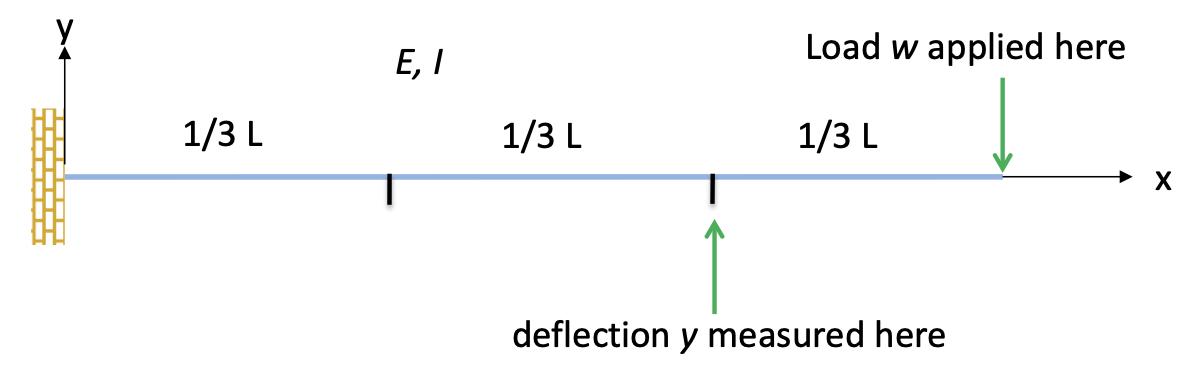
\includegraphics[width=6in]{images/Config 1-3}
\caption{The beam configuration for experiments 1--3.}
\label{fig:config_1-3}
\end{figure}

Table \ref{tbl:configs} summarizes the differences between configurations 1--3.

\begin{table}[!htbp]
\caption{Dimensions and loads for configurations 1--3.}
\begin{center}
	\begin{tabular}{|c|c|c|c|c|}
		\hline
		Config&Base, $b$ [\unit{\mm}]&Height, $h$ [\unit{\mm}]&Mass [\unit{\g}]&Weight [\unit{\N}]\\
		\hline
		\num{1}&\num{12.8}&\num{6.4}&\num{100}&\num{0.981}\\
		\hline
		\num{2}&\num{6.4}&\num{12.8}&\num{200}&\num{1.96}\\
		\hline
		\num{3}&\num{12.8}&\num{12.8}&\num{500}&\num{4.905}\\
		\hline
	\end{tabular}
\end{center}
\label{tbl:configs}
\end{table}

For configuration 4, shown in Figure \ref{fig:config_4}, the beam was fixed at one end and---measuring from the fixed end---a roller was positioned at $x=L$, a load was applied at $x=\frac{1}{3}L$, and the deflection was measured at $x=\frac{2}{3}L$. The rectangular beam (\qtyproduct{12.8x6.4}{\mm}) was used, and the mass was \qty{1000}{\g}, resulting in a \qty{9.81}{\N} load.

\begin{figure}[htbp]
\centering
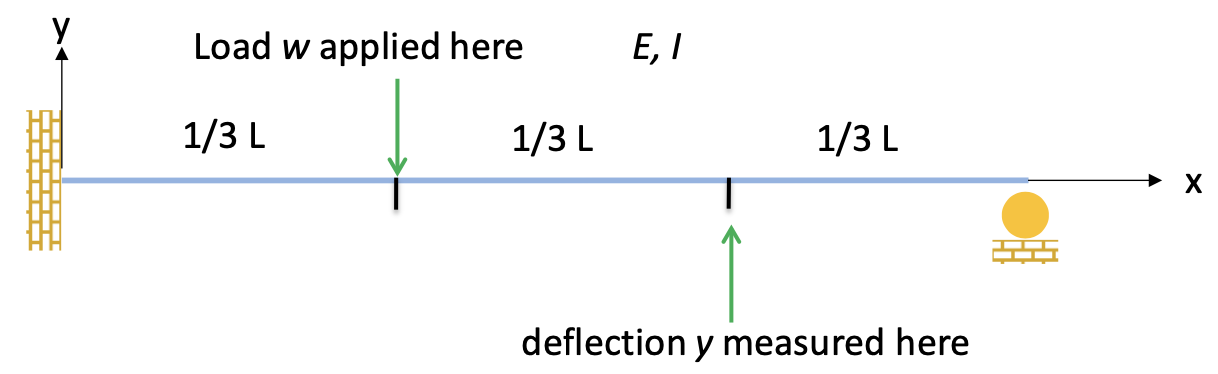
\includegraphics[width=6in]{images/Config 4}
\caption{The beam configuration for experiment 4.}
\label{fig:config_4}
\end{figure}

For configuration 5, shown in Figure \ref{fig:config_5}, the beam was fixed at one end and---measuring from the fixed end---a roller was positioned at $x=\frac{2}{3}L$, mass $m_1$ was applied at $x=\frac{1}{3}L$, mass $m_2$ was applied at $x=L$, and the deflection was measured at $x=L$. The rectangular beam (\qtyproduct{12.8x6.4}{\mm}) was used. Mass $m_1$ was \qty{2500}{\g}, resulting in a \qty{24.5}{\N} load, and mass $m_2$ was \qty{200}{\g}, resulting in a \qty{1.96}{\N} load.

\begin{figure}[htbp]
\centering
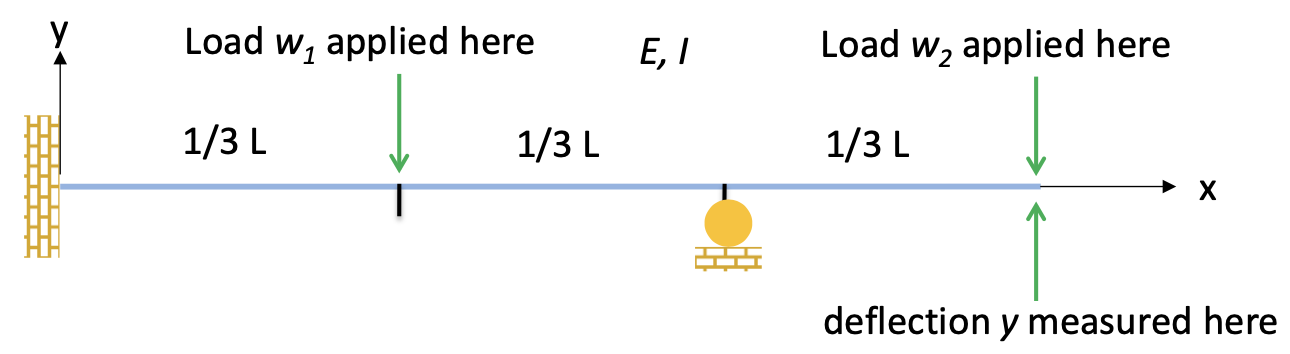
\includegraphics[width=6in]{images/Config 5}
\caption{The beam configuration for experiment 5.}
\label{fig:config_5}
\end{figure}

\section{Procedures} \label{procedures}
Before measuring any deflections, ensure the testing table is level by using the level gauge. If the table is not level, adjust the bench legs with the provided wrench. For configurations 1--2 and 3--4, clamp the rectangular beam to the wood board according to the dimensions shown in Table \ref{tbl:configs}. For configuration \num{3}, use the square beam (see Figure \ref{fig:config_3_img}). Level the beam with the leveling gauge. Ensure the beam length sticking out past the wooden board is \qty{90}{\cm} as described in Section \ref{apparatus}. For configurations 4--5, position the wooden roller underneath the beam at the locations described in Section \ref{apparatus}.

\begin{figure}[htbp]
\centering
\includegraphics[width=4in]{images/Config C}
\caption{Configuration \num{3} fully configured and ready for the weights to be applied.}
\label{fig:config_3_img}
\end{figure}

Set up the PASCO displacement needle at the location prescribed in Section \ref{apparatus}. For configurations 1--4, the displacement needle should be underneath the beam pointing upwards. For configuration \num{5}, the needle should be above the beam pointing downwards (see Figure \ref{fig:config_5_img}). Before each measurement, zero the displacement needle. Add the appropriate masses at the described locations (see Section \ref{apparatus}) and record the displacement. For each configuration, take three measurements and calculate the mean displacement of the three measurements. Repeat these steps for each of the five configurations.

\begin{figure}[htbp]
\centering
\includegraphics[width=4in]{images/Config E}
\caption{Configuration \num{5} fully configured and ready for the weights to be applied. Note the orientation of the displacement needle.}
\label{fig:config_5_img}
\end{figure}

\section{Data} \label{data}
The displacements in lab were recorded with the digital displacement gauge. The values are tabulated in Table \ref{tbl:data}.

\begin{table}[!htbp]
\caption{Tabulated displacements in the five different beam configurations.}
\begin{center}
	\begin{tabular}{|c|c|c|c|c|}
		\hline
		Config&Meas. 1 [\unit{\mm}]&Meas. 2 [\unit{\mm}]&Meas. 3 [\unit{\mm}]&Avg [\unit{\mm}]\\
		\hline
		\num{1}&\num{-4.62}&\num{-4.59}&\num{-4.60}&\num{-4.60}\\
		\hline
		\num{2}&\num{-3.55}&\num{-3.59}&\num{-3.57}&\num{-3.57}\\
		\hline
		\num{3}&\num{-5.01}&\num{-5.10}&\num{-5.00}&\num{-5.04}\\
		\hline
		\num{4}&\num{-2.13}&\num{-2.11}&\num{-2.12}&\num{-2.12}\\
		\hline
		\num{5}&\num{2.37}&\num{2.37}&\num{2.22}&\num{2.32}\\
		\hline
	\end{tabular}
\end{center}
\label{tbl:data}
\end{table}

\section{Analysis} \label{analysis}
To derive the following deflection expressions, we are given the following equations of superposition for a cantilever beam:
\begin{align}
	0\le{}x\le{}L_1:y&=-\frac{wx^2}{6EI}(3L_1-x)\label{eqn:superpos_1}\\
	L_1\le{}x\le{}L:y&=-\frac{wL_1^2}{6EI}(3x-L_1)\label{eqn:superpos_2}\\
	L_1=L:y&=-\frac{wx^2}{6EI}(3L-x)\label{eqn:superpos_3}
\end{align}
where $L$ is the length of the beam, $E$ is the elastic modulus of the beam material, $I$ is the beam moment of inertia, $w$ is the applied load, $L_1$ is the distance from the fixed end of the beam to the applied load, and $x$ is the point about which deflection is measured. Note that Equation \ref{eqn:superpos_2} is invalid for $L_1=L$.

The configuration for test four, shown in Figure \ref{fig:config_4}, consists of a beam fixed at one end with a roller support on the other end. A load is being applied at $\frac{1}{3}$ the length, measured from the fixed end. To calculate the deflection at $\frac{2}{3}$ the length, \ie $x=\frac{2}{3}L$, we are given the following equation:
\begin{align} \label{eqn:config_4-deflection}
	\nu&=-\frac{w}{EI}\frac{23}{4374}L^3
\end{align}
where $w$ is the applied load, $E$ is the elastic modulus, $I$ is the moment of inertia, $L$ is the length of the beam, and $\nu$ is the deflection of the beam at $x=\frac{2}{3}L$.

To derive this expression, we first note that the beam configuration is indeterminate. The roller support is redundant and can be replaced by a vertical applied load of magnitude $R_y$. The beam is now effectively a cantilevered beam with two applied loads. Deflection at a point $x$ can be calculated by summing the deflection at $x$ from each of the applied loads.

The deflection due to the applied load at $x=\frac{1}{3}L$, $\nu_w$, can be derived from Equation \ref{eqn:superpos_2}.
\begin{align*}
	\nu_w(x)&=-\frac{wL_1^2}{6EI}(3x-L_1)\\
	&=-\frac{w\frac{1}{9}L^2}{6EI}(3x-\frac{1}{3}L)\\
	&=-\frac{wL^2}{162EI}(9x-L)
\end{align*}
This expression is true for all $x\in[\frac{1}{3}L,L]$.

The deflection due to the redundant reaction force at $x=L$, $\nu_{R_y}$, can be derived from Equation \ref{eqn:superpos_3}.
\begin{align*}
	\nu_{R_y}(x)&=-\frac{wx^2}{6EI}(3L-x)\\
	&=-\frac{R_yx^2}{6EI}(3L-x)
\end{align*}
This expression is true for all $x\in[0,L]$.

To calculate the deflection at $x=\frac{2}{3}L$, we first need to determine the value of $R_y$. We know from Figure \ref{fig:config_4}, at $x=L$ there is a roller support, and therefore, $\nu(x)=0$ at $x=L$. We apply this boundary condition below to find $R_y$.
\begin{align*}
	\nu(L)&=\nu_w(L)+\nu_{R_y}(L)=0\\
	0&=-\frac{wL^2}{162EI}(9L-L)-\frac{R_yL^2}{6EI}(3L-L)\\
	0&=-\frac{4wL^3}{81EI}-\frac{R_yL^3}{3EI}\\
	R_y&=-\frac{4w}{27}
\end{align*}
Substituting in the derived expression for $R_y$ into the earlier equation for $\nu_{R_y}$, we find that
\begin{align*}
	\nu_{R_y}(x)&=\frac{2wx^2}{81EI}(3L-x)
\end{align*}
Now that we have expressions for both $\nu_w$ and $\nu_{R_y}$ in terms of $w$, we can find the derive an equation for the deflection of the beam at $x=\frac{2}{3}L$ in terms of $w$, $E$, $I$, and $L$.
\begin{align*}
	\nu\left(\frac{2}{3}L\right)&=\nu_w\left(\frac{2}{3}L\right)+\nu_{R_y}\left(\frac{2}{3}L\right)\\
	&=-\frac{wL^2}{162EI}\left(9\left(\frac{2}{3}L\right)-L\right)+\frac{2w\left(\frac{2}{3}L\right)^2}{81EI}\left(3L-\left(\frac{2}{3}L\right)\right)\\
	&=-\frac{5wL^3}{162EI}+\frac{56wL^3}{2187EI}\\
	&=\frac{wL^3}{EI}\left(-\frac{5}{162}+\frac{56}{2187}\right)\\
	&=-\frac{23wL^3}{4374EI}
\end{align*}
As expected, this equation matches the given expression in Equation \ref{eqn:config_4-deflection}. Calculating the theoretical deflection is then trivial. We know $w=(\qty{1000}{\g})(\frac{\qty{1}{\kg}}{\qty{1000}{\g}})(\qty[per-mode=fraction]{9.81}{\m\per\s\squared})=\qty{9.81}{\N}$, $L=\qty{0.90}{\m}$, $E=\qty{68.9e9}{\Pa}$, and $I=\frac{1}{12}(\qty{12.8}{\mm})(\qty{6.4}{\mm})^3(\frac{\qty{1}{\m}}{\qty{1000}{\mm}})^4=\qty{2.796e-10}{\m^4}$. Plugging these values into Equation \ref{eqn:config_4-deflection}, we find that
\begin{align*}
	\nu\left(\frac{2}{3}L\right)&=-\frac{23(\qty{9.81}{\N})(\qty{0.90}{\m})^3}{4374(\qty{68.9e9}{\Pa})(\qty{2.796e-10}{\m^4})}\\
	&=\qty{-1.952}{\mm}\text{ or }\qty{1.952}{\mm}\downarrow
\end{align*}

The configuration for test five, shown in Figure \ref{fig:config_5}, consists of a beam fixed at one end with a roller support at $\frac{2}{3}$ the length. A load is being applied at $\frac{1}{3}$ the length and at the end, measured from the fixed end. To calculate the deflection at the free end of the beam, \ie $x=L$, we are given the following equation:
\begin{align} \label{eqn:config_5-deflection}
	\nu&=-\frac{L^3}{EI}\left(\frac{5w_2}{162}-\frac{w_1}{216}\right)
\end{align}
where $w_1$ is the applied load at $x=\frac{1}{3}L$, $w_2$ is the applied load at $x=L$, $E$ is the elastic modulus, $I$ is the moment of inertia, $L$ is the length of the beam, and $\nu$ is the deflection of the beam at $x=L$.

To derive this expression, we first note that the beam configuration is indeterminate. The roller support is redundant and can be replaced by a vertical applied load of magnitude $R_y$. The beam is now effectively a cantilevered beam with three applied loads. Deflection at a point $x$ can be calculated by summing the deflection at $x$ from each of the applied loads.

The deflection due to the applied load at $x=\frac{1}{3}$, $\nu_{w_1}$, can be derived from Equation \ref{eqn:superpos_2}.
\begin{align*}
	\nu_{w_1}(x)&=-\frac{wL_1^2}{6EI}(3x-L_1)\\
	&=-\frac{w_1\frac{1}{9}L^2}{6EI}(3x-\frac{1}{3}L)\\
	&=\frac{w_1L^2}{162EI}(9x-L)
\end{align*}
This expression is true for all $x\in[\frac{1}{3}L,L]$.

The deflection due to the redundant reaction force at $x=\frac{2}{3}L$, $\nu_{R_y}$, can be derived from Equation \ref{eqn:superpos_2}.
\begin{align*}
	\nu_{R_y}(x)&=-\frac{wL_1^2}{6EI}(3x-L_1)\\
	&=-\frac{R_y\frac{4}{9}L^2}{6EI}(3x-\frac{2}{3}L)\\
	&=-\frac{2R_yL^2}{81EI}(9x-2L)
\end{align*}
This expression is true for all $x\in[\frac{2}{3}L,L]$.

The deflection due to the applied load at $x=L$, $\nu_{w_2}$, can be derived from Equation \ref{eqn:superpos_3}.
\begin{align*}
	\nu_{w_2}(x)&=-\frac{wx^2}{6EI}(3L-x)\\
	&=-\frac{w_2}x^2{6EI}(3L-x)
\end{align*}
This expression is for all $x\in[0,L]$.

To calculate the deflection at $x=L$, we first need to determine the value of $R_y$. We know from Figure \ref{fig:config_5}), at $x=\frac{2}{3}L$ there is a roller support, and therefore, $\nu(x)=0$ at $x=\frac{2}{3}L$. We apply this boundary condition below to find $R_y$.
\begin{align*}
	\nu(\frac{2}{3}L&=\nu_{w_1}(\frac{2}{3}L)+\nu_{R_y}(\frac{2}{3}L)+\nu_{w_2}(\frac{2}{3}L)=0\\
	0&=-\frac{w_1L^2}{162EI}(9(\frac{2}{3}L)-L)-\frac{2R_yL^2}{81EI}(9(\frac{2}{3}L)-2L)-\frac{w_2\frac{4}{9}L^2}{6EI}(3L-(\frac{2}{3}L)\\
	0&=-\frac{5w_1}{162}-\frac{8R_y}{81}-\frac{14w_2}{81}\\
	R_y&=-\frac{5}{16}(w_1+\frac{28w_2}{5})	
\end{align*}
Now that we have expressions for the deflection due to all the forces, we can derive an equation for the deflection of the beam at $x=L$ using the method of superposition.
\begin{align*}
	\nu(L)&=\nu_{w_1}(L)+\nu_{R_y}(L)+\nu_{w_2}(L)\\
	&=-\frac{w_1L^2}{162EI}(9L-L)-\frac{2\left(-\frac{5}{16}\left[w_1+\frac{28w_2}{5}\right]\right)L^2}{81EI}(9L-2L)-\frac{w_2L^2}{6EI}(3L-L)\\
	&=-\frac{4w_1L^3}{81EI}+\frac{35\left(w_1+\frac{28w_2}{5}\right)L^3}{648EI}-\frac{w_2L^3}{3EI}\\
	&=-\frac{L^3}{EI}\left[\frac{4w_1}{81}-\frac{35w_1}{648}-\frac{49w_2}{162}+\frac{w_2}{3}\right]\\
	&=-\frac{L^3}{EI}\left(\frac{5w_2}{162}-\frac{w_1}{216}\right)
\end{align*}
As expected, this equation matches the given expression in Equation \ref{eqn:config_5-deflection}. Calculating the theoretical deflection is then trivial. We know $w_1=(\qty{2500}{g})(\frac{\qty{1}{kg}}{\qty{1000}{\g}})(\qty[per-mode=fraction]{9.81}{\m\per\s\squared})=\qty{24.53}{\N}$, $w_2=(\qty{200}{\g})(\frac{\qty{1}{\kg}}{\qty{1000}{\g}})(\qty[per-mode=fraction]{9.81}{\m\per\s\squared})=\qty{1.962}{\N}$, $L=\qty{0.90}{\m}$, $E=\qty{68.9e9}{\Pa}$, and $I=\frac{1}{12}(\qty{12.8}{\mm})\cdot(\qty{6.4}{\mm})^3(\frac{\qty{1}{\m}}{\qty{1000}{\mm}})^4=\qty{2.796e-10}{\m^4}$. Plugging these values into Equation \ref{eqn:config_5-deflection}, we find that
\begin{align*}
	\nu(L)&=-\frac{\qty{0.90}{\m}}{(\qty{68.9e9}{\Pa})(\qty{2.796e-10}{\m^4})}\left(\frac{5(\qty{1.962}{\N})}{162}-\frac{\qty{24.53}{\N}}{216}\right)\\
	&=\qty{2.475}{\mm}\text{ or }\qty{2.475}{\mm}\uparrow
\end{align*}

Using the theoretical values calculated above and during prelab, Table \ref{tbl:compare} compares the theoretical deflections to the deflections measured in lab. The deflections measured in lab are an average of three measurements. A negative deflection implies deflection is towards the ground ($\downarrow$).

\begin{table}[!htbp]
\caption{Theoretical and measured beam deflections for the five configurations in lab.}
\begin{center}
	\begin{tabular}{|c|c|c|c|}
		\hline
		Configuration&Theoretical [\unit{\mm}]&Measured [\unit{\mm}]&Error\\
		\hline
		1&\num{-6.416}&\num{-4.60}&\qty{28.3}{\percent}\\
		\hline
		2&\num{-3.208}&\num{-3.57}&\qty{11.3}{\percent}\\
		\hline
		3&\num{-4.010}&\num{-5.04}&\qty{25.6}{\percent}\\
		\hline
		4&\num{-1.952}&\num{-2.12}&\qty{8.61}{\percent}\\
		\hline
		5&\num{2.475}&\num{2.32}&\qty{6.30}{\percent}\\
		\hline
	\end{tabular}
\end{center}
\label{tbl:compare}
\end{table}

Two of the configurations, configuration one and configuration three, had particularly high error. For configuration one, this error was likely caused by the smaller surface area exposed to the clamp. In configuration one, the height of the surface the clamp was attached to was \qty{6.4}{\mm} rather than \qty{12.8}{\mm}. This made it very difficult to attach the beam to the board with the clamp, and it is likely that throughout the tests, the beam may have become unstable or unlevel. We noticed in this configuration specifically that the beam would twist slightly under the force of the mass. In configuration three, there was quite a lot of weight on the end of the cantilevered beam with only a clamp fixing the beam to the board. It is very possible the beam was slipping from the clamp under the \qty{500}{\g} mass.

The other tests matched the theoretical values quite well. These amounts of error on such a small scale could be attributed to the accuracy of the device. We have shown in previous labs that the displacement needle is not the most precise or accurate measuring device, and when the scale of displacement is in the single digit millimeters, error of \qtyrange{6}{16}{\percent} is expected without precise equipment.

It is also possible the weights were not exactly the correct mass, the weights were not placed at exactly the correct location---\ie the measurements on the beam may have been off by several millimeters or more---or the aluminum beam we used could have had a higher or lower Young's Modulus than the theoretical value. Any of these reasons could have contributed to the displacement being off by several millimeters.

\section{Conclusion} \label{conclusion}
Our hypothesis generally held true. The theoretical measurements were different from the measured values. The lowest recorded error was for configuration five (\qty{6.30}{\percent} error) and the highest recorded error was for configuration one (\qty{28.3}{\percent}. Configuration one had higher error than expected, likely due to the low clamping surface area. Configuration three also had high error, likely due to the large mass and minimal cantilevering support. The measuring equipment and the superposition approximation both contributed to error, but were not significant sources of error.

Despite the error, we were able to show that the method of superposition is an accurate and powerful tool for calculating beam deflection if extremely high accuracy is not required. The theoretical values were all in the same order of magnitude and the in the same direction as the measured values.
\end{document}
